\chapter{Constraining {\sc Galacticus}}

\section{Optimal Halo Mass Function Sampling}

Suppose we want to fit parameters of the \glc\ model to some dataset. The basic approach is to generate large numbers of model realizations for different parameter values and see which ones best match the data. \glc\ models involve simulating individual merger trees and then adding together their galaxies to produce some overall function. The question we want to answer is, given some finite amount of computing time, what is the optimal distribution of halo masses to run when comparing to a given dataset. For example, is it better to run a volume limited sample (as one would get from an N-body simulation) or is it better to use, say, equal numbers of halos per logarithmic interval of halo mass? The following section describes how to solve this optimization problem in the specific case of fitting to the stellar mass function.

\subsection{Li \& White (2009) Stellar Mass Function}\label{sec:OptimalSamplingStellarMassFunction}

 First, some definitions:
\begin{description}
 \item [$n(M) \d \ln M$] is the dark matter halo mass function, i.e. the number of halos in the range $M$ to $M+M\d\ln  M$ per unit volume;
 \item [$\gamma(M) \d \ln M$] is the number of trees that we will simulate in the range $M$ to $M+M\d \ln M$;
 \item [$\alpha(M_\star)$] is the error on the observed stellar mass function at mass $M_\star$;
 \item [$P(N|M_\star,M;\delta \ln M_\star)$] is the conditional stellar mass distribution function of galaxies of stellar mass $M_\star$ in a bin of width $\delta \ln M_\star$ per halo of mass $M$;
 \item [$t(M)$] is the CPU time it takes to simulate a tree of mass $M$.
\end{description}
To clarify, $P(N|M_\star,M;\delta \ln M_\star;\delta \ln M_\star)$ is the probability\footnote{To put it another way, $P(N|M_\star,M;\delta \ln M_\star)$ is closely related to the commonly used Halo Occupation Distribution.} to find $N$ galaxies of mass between $M_\star$ in a bin of width $\delta \ln M_\star$ in a halo of mass $M$. The usual conditional stellar mass function is simply the first moment of this distribution:
\begin{equation}
 \phi(M_\star;M) \delta \ln M_\star = \sum_{N=0}^\infty N P(N|M_\star,M;\delta \ln M_\star)
 \label{eq:cSMFdefinition}
\end{equation}
The model estimate of the stellar mass function $\Phi(M_\star)$ (defined per unit $\ln M_\star$) is
\begin{equation}
 \Phi(M_\star) = \int_0^\infty \phi(M_\star;M) {n(M) \over \gamma(M)} \gamma(M) \d \ln M,
\end{equation}
where the $n(M)/\gamma(M)$ term is the weight assigned to each tree realization---and therefore the weight assigned to each model galaxy when summing over a model realization to construct the stellar mass function. 

When computing a model likelihood, we must employ some statistic which defines how likely the model is given the data. Typically, for stellar mass functions we have an estimate of the variance in the data, $\alpha^2(M_\star)$, as a function of stellar mass (full covariance matrices are typically not provided but, ideally would be, and can be easily incorporated into this method). In that case, we can define a likelihood
\begin{equation}
 \ln \mathcal{L} = - {1 \over 2} \sum_i {[\phi_{{\rm obs},i} - \phi_i]^2 \over \alpha_i^2 + \sigma_i^2}
\end{equation}
where the sum is taken over all data points, $i$, and $\sigma_i^2$ is the variance in the model estimate and is given by
\begin{equation}
 \sigma^2(M_\star) = \langle [\phi(M_\star) - \bar{\phi}(M_\star)]^2 \rangle,
\end{equation}
where $\phi(M_\star)$ is the realization from a single model and $\bar{\phi}(M_\star)$ is the model expectation from an infinite number of merger tree realizations and the average is taken over all possible model realizations. Since the contributions from each merger tree are independent, 
\begin{equation}
 \sigma^2(M_\star) = \sum_i \zeta_i^2(M_\star;M)
\end{equation}
where $\zeta_i^2(M_\star;M)$ is the variance in the contribution to the stellar mass function from tree $i$. This in turn is given by
\begin{equation}
 \zeta^2(M_\star;M) = \psi^2(M_\star;M) \left[{n(M) \over \gamma(M)}\right]^2,
\end{equation}
where $\psi^2(M_\star;M)$ is the variance in the conditional stellar mass function. In the continuum limit this becomes
\begin{equation}
 \sigma^2(M_\star) = \int_0^\infty \psi^2(M_\star;M) \left[{n(M) \over \gamma(M)}\right]^2 \gamma(M) \d \ln M.
\end{equation}

Model variance artificially increases the likelihood of a given model. We would therefore like to minimize the increase in the likelihood due to the model variance:
\begin{equation}
\Delta 2 \ln \mathcal{L} = \sum_i {[\phi_{{\rm obs},i} - \phi_i]^2 \over \alpha_i^2} - {[\phi_{{\rm obs},i} - \phi_i]^2 \over \alpha_i^2 + \sigma_i^2} 
\end{equation}
Of course, we don't know the model prediction, $\phi_i$, in advance\footnote{Below, we will adopt a simple empirical model for $\phi(M_\star)$. However, it should not be used here since we will in actuality be computing the likelihood from the model itself.}. However, if we assume that a model exists which is a good fit to the data then we would expect that $[\phi_{{\rm obs},i} - \phi_i]^2 \approx \alpha_i^2$ on average. In that case, the increase in likelihood due to the model is minimized by minimizing the function\footnote{This can be seen intuitively: we are simply requring that the variance in the model prediction is small compared the the variance in the data.}
\begin{equation}
 F[\gamma(M)] = \sum_i {\alpha_i^2 \over \alpha_i^2 + \sigma_i^2}.
\end{equation}
If the bins all have the same $\delta \ln M_\star$ we can turn the sum into an integral
\begin{equation}
 F[\gamma(M)] = \int_0^\infty {\alpha(M_\star)^2 \over \alpha(M_\star)^2 + \sigma(M_\star)^2} \d \ln M_\star.
\end{equation}
Obviously, the answer is to make $\gamma(M)=\infty$, in which case $ F[\gamma(M)]=0$. However, we have finite computing resources. The total time to run our calculation is
\begin{equation}
 \tau = \int_0^\infty t(M) \gamma(M) \d \ln M.
\end{equation}
We therefore want to minimize $F[\gamma(M)]$ while keeping $\tau$ equal to some finite value. We can do this using a Lagrange multiplier and minimizing the function
\begin{equation}
  F[\gamma(M)] = \int_0^\infty {\alpha(M_\star)^2 \over \alpha(M_\star)^2 + \sigma(M_\star)^2} \d \ln M_\star + \int_0^\infty \lambda \gamma(M) t(M) \d \ln M.
\end{equation}
Finding the functional derivative and setting it equal to zero gives:
\begin{equation}
 \gamma(M) = \sqrt{{\xi(M) \over \lambda t(M)}},
\end{equation}
in the limit where\footnote{This is the limit in which we would like our results to be.} $\sigma(M_\star) \ll \alpha(M_\star)$, and where
\begin{equation}
 \xi(M) = n^2(M) \int_{-\infty}^\infty {\psi^2(M_\star;M) \over \alpha^2(M_\star)} \d \ln M_\star.
\end{equation}
The values of $\lambda$ and $\delta \ln M_\star$, and the normalization of $t(M)$ are unimportant here since we merely want to find the optimal shape of the $\gamma(M)$ function---we can then scale it up or down to use the available time.

Figure~\ref{fig:optimalSamplingStellarMassFunction} shows the function $\gamma(M)$ obtained by adopting a model conditional stellar mass function which is a sum of central and satellite terms. Specifically, we use the model of \cite{leauthaud_new_2011} which is constrained to match observations from the COSMOS survey. In their model\footnote{This integral form of the conditional stellar mass function is convenient here since it allows for easy calcualtion of the number of galaxies expected in the finite-width bins of the observed stellar mass function.}:
\begin{equation}
 \langle N_{\rm c}(M_\star|M)\rangle \equiv \int_{M_\star}^\infty \phi_{\rm c}(M_\star^\prime) \d \ln M_\star^\prime = {1 \over 2} \left[ 1 - \hbox{erf}\left( {\log_{10}M_\star - \log_{10} f_{\rm SHMR}(M) \over \sqrt{2}\sigma_{\log M_\star}} \right) \right].
\end{equation}
Here, the function $f_{\rm SHMR}(M)$ is the solution of
\begin{equation}
 \log_{10}M = \log_{10}M_1 + \beta \log_{10}\left({M_\star \over M_{\star,0}}\right) + {(M_\star/M_{\star,0})^\delta \over 1 + (M_\star/M_{\star,0})^{-\gamma}} - {1/2}.
\end{equation}
For satellites,
\begin{equation}
 \langle N_{\rm s}(M_\star|M)\rangle \equiv \int_{M_\star}^\infty \phi_{\rm s}(M_\star^\prime) \d \ln M_\star^\prime =  \langle N_{\rm c}(M_\star|M)\rangle \left({f^{-1}_{\rm SHMR}(M_\star) \over M_{\rm sat}}\right)^{\alpha_{\rm sat}} \exp\left(- {M_{\rm cut} \over f^{-1}_{\rm SHMR}(M_\star)} \right),
\end{equation}
where
\begin{equation}
 {M_{\rm sat} \over 10^{12} M_\odot} = B_{\rm sat} \left({f^{-1}_{\rm SHMR}(M_\star) \over 10^{12} M_\odot}\right)^{\beta_{\rm sat}},
\end{equation}
and
\begin{equation}
 {M_{\rm cut} \over 10^{12} M_\odot} = B_{\rm cut} \left({f^{-1}_{\rm SHMR}(M_\star) \over 10^{12} M_\odot}\right)^{\beta_{\rm cut}}.
\end{equation}

We use the best fit parameters from the {\tt SIG\_MOD1} method of \cite{leauthaud_new_2011} for their $z_1$ sample, but apply a shift of $-0.2$ dex in masses to bring the fit into line with the $z=0.07$ mass function of \cite{li_distribution_2009}. The resulting parameter values are shown in Table~\ref{tb:z0SMFFitParameters}.

\begin{table}
\begin{center}
\caption{Parameters of the conditional stellar mass function fit.}
\label{tb:z0SMFFitParameters}
\begin{tabular}{lr@{.}lr@{.}l}
\hline
{\bf Parameter} & \multicolumn{2}{c}{\bf Value} \\
\hline
$\alpha_{\rm sat}$& 1&0 \\
$\log_{10} M_1$& 12&120 \\
$\log_{10} M_{\star,0}$& 10&516 \\
$\beta$& 0&430 \\
$\delta$& 0&5666 \\
$\gamma$& 1&53 \\
$\sigma_{\log M_\star}$& 0&206 \\
$B_{\rm cut}$& 0&744 \\
$B_{\rm sat}$& 8&00 \\
$\beta_{\rm cut}$& $-$0&13 \\
$\beta_{\rm sat}$& 0&859 \\
\hline
\end{tabular}
\end{center}
\end{table}

We assume that $P_{\rm s}(N|M_\star,M;\delta \ln M_\star)$ is a Poisson distribution while $P_{\rm c}(N|M_\star,M;\delta \ln M_\star)$ has a Bernoulli distribution, with each distribution's free parameter fixed by the constraint of eqn.~(\ref{eq:cSMFdefinition}), and the assumed forms for $\phi_{\rm c}$ and $\phi_{\rm s}$.

The errors in the \cite{li_distribution_2009} observed stellar mass function are well fit by (see Fig.~\ref{fig:stellarMassFunctionErrors}):
\begin{equation}
 \alpha(M_\star) = 10^{-3} \left({M_\star\over 4.5\times 10^{10}M_\odot}\right)^{-0.3} \exp\left(-{M_\star\over 4.5\times 10^{10}M_\odot}\right) + 10^{-7},
 \label{eq:stellarMassFunctionErrorsFit}
\end{equation}
and the tree processing time in \glc\ can be described by:
\begin{equation}
 \log_{10} t(M) = \sum_{i=0}^2 C_i [ \log_{10} M ]^i
\end{equation}
with $C_0=-0.73$, $C_1=-0.20$ and $C_2=0.035$.

The resulting optimal sampling density curve is shown in Fig.~\ref{fig:optimalSamplingStellarMassFunction} and is compared to weighting by the halo mass function (i.e. the result of sampling halos at random from a representative volume). Optimal sampling gives less weight to low mass halos (since a sufficient accuracy can be obtained without the need to run many tens of thousands of such halos) and to high mass halos which are computationally expensive. 

\begin{figure}
 \begin{center}
 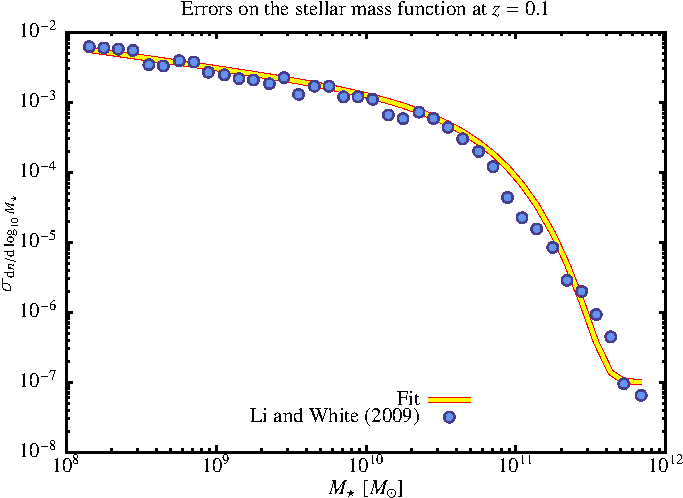
\includegraphics[width=160mm]{../plots/stellarMassFunctionErrors_z01.pdf}
 \end{center}
 \caption{Errors on the \protect\cite{li_distribution_2009} stellar mass funtion (points) and the fitting function (line) given by eqn.~(\protect\ref{eq:stellarMassFunctionErrorsFit}).}
 \label{fig:stellarMassFunctionErrors}
\end{figure}

\begin{figure}
 \begin{center}
 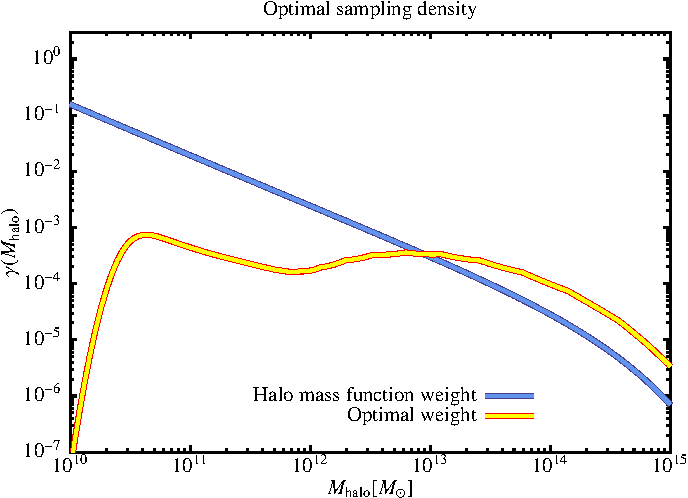
\includegraphics[width=160mm]{../plots/optimalSamplingStellarMassFunction.pdf}
 \end{center}
 \caption{Optimal weighting (yellow line) compared with weighting by the dark matter halo mass function (i.e. sampling halos at random from a representative volume; blue line). Sampling densities have been normalized to unit compute time.}
 \label{fig:optimalSamplingStellarMassFunction}
\end{figure}

\subsection{Refining by Other Merger Tree Statistics}

Since building merger trees is relatively fast, while solving the baryonic physics is slow it may be advantageous to  non-uniformly sample the distribution of merger trees at fixed merger tree mass, $M$. For example, we could assign some measure of formation history to each merger tree, such as the time since the last major merger, $\tau$. The halo mass function then becomes $n(M,\tau)$ (which can be computed by simulating large numbers of trees), and the tree sampling function becomes $\gamma(M,\tau)$. We'd then need to know the stellar mass function conditioned on both $M$ and $\tau$, $\phi_\star(M_\star|M,\tau)$. Given these, the above approach could be easily generalized to determine an optimal $\gamma(M,\tau)$. Then, after generating a merger tree, we'd first compute $\tau$. If a sufficient number of trees in that $\tau$ interval had already been computed, then we'd simply drop that tree and compute another one. The speed up here would depend on how fast building trees is relative to solving baryonic physics and what fraction of trees you discard. In principle, the trees could be generated, sampled and stored in advance so that we'd already have an optimally distributed set of trees in $M$ and $\tau$ that could be used for each model run.
